%%%%%%%%%%%%%%%%%%%%%%%%%%%%%%%%%%%%%%%%%%%%%%%%%%%%%%%%%%%%%%%%%%%%%%%%%%%%%

\chapter{La sonate op. 27}

La sonate op.27 en \emph{fa} mineur a été composée entre 1906 et 1908. Publiée en novembre 1908 par Julius Heinrich Zimmermann à Leipzig, cette œuvre compte parmi les plus fameuses du compositeur. Elle est dédié à Karl Klindworth, l'ancien professeur de piano de Liapounov du temps où il étudiait au conservatoire de Moscou. Cette sonate présente un intéret autant par sa forme et ses qualités musicales que par son écriture pianistique. Sa structure complexe la rapproche des concertos ou de la célèbre sonate en \emph{si} mineur S.178 de Liszt.

Comme l'atteste l'importante correspondance entretenue avec Balakirev, Klindworth, Zimmermann, Villoing, et Viñes, l'écriture de cette œuvre s'avère difficile. C'est une période où Liapounov travaille beaucoup. En plus de la sonate, il compose simultanément sa \emph{Rhapsodie sur des thèmes ukrainiens} op.28, sa transcription pour piano du \emph{Pogibnet} de l'opéra \emph{Ruslan et Ludmila} de Glinka et ses \emph{Deux pièces pour piano} op.33, paraphrases du même opéra. Il effectue de plus ses premiers concerts à Berlin et Leipzig en 1907 auquels il faut ajouter une importante représentation à Moscou.\\

Dans ce chapitre, nous proposons une modeste analyse de cette imposante sonate.

\section{Premières constatations}

L'œuvre ne contient qu'un seul grand mouvement d'environ 31 pages pour 25 minutes de musique. On pense directement à la sonate en \emph{si} mineur S.178 de Liszt qui a exactement les même dimensions soit environ 33 pages pour 25 minutes de musique. En observant plus attentivement la partition, nous distinguons très clairement la présences de quatre parties enchaînées sans interruption du discours musical :
\begin{enumerate}
  \item Allegro appassionato (C), mesures 1 à 244.
  \item Andante sostenuto e molto espressivo (12/8), mesures 245 à 362.
  \item Allegro vivo, scherzando (6/8), mesures 363 à 454.
  \item Tempo I (C), mesures 455 à 598.\\
\end{enumerate}

Nous retrouvons la structure traditionnelle d'une sonate à quatre mouvements à savoir un mouvement rapide, un mouvement lent, un scherzo et un finale.\\

La seconde constatation, est la présences de cinq thèmes évoluants tout au long de l'œuvre.\\

\textbf{Le premier (thème A)}, apparaît page 1, mesure 1 au \emph{Allegro appassionato} (voir figure \ref{sonate-theme-1}). Écrit à quatre temps, dans l'obscure tonalité de \emph{fa} mineur, il s'agit d'un thème rythmé (croches pointées doubles) et expressif. Les premières notes de tête \emph{do} \emph{si}$\natural$ \emph{do} (\emph{fa}) \emph{la}$\flat$ évoquent peut-être le \emph{Dies iræ}. Mesures 2 et 3, remarquons aussi la ligne descendante de la basse \emph{ré}$\flat$ \emph{do} \emph{si}$\flat$ \emph{la}$\flat$ \emph{sol} \emph{sol}$\flat$ \emph{fa} \emph{mi}$\flat$ \emph{ré}$\flat$ et des voix intérieures qui émergent des cinq premières notes. La seconde partie du thème est en \emph{ré}$\flat$ majeur. Les troisième et quatrièmes notes forment une quarte au lieu de la quinte initiale.

\begin{figure}[!ht]
  \begin{bigcenter}
    \vspace*{0.2cm}
    \begin{tabular}{lr}
      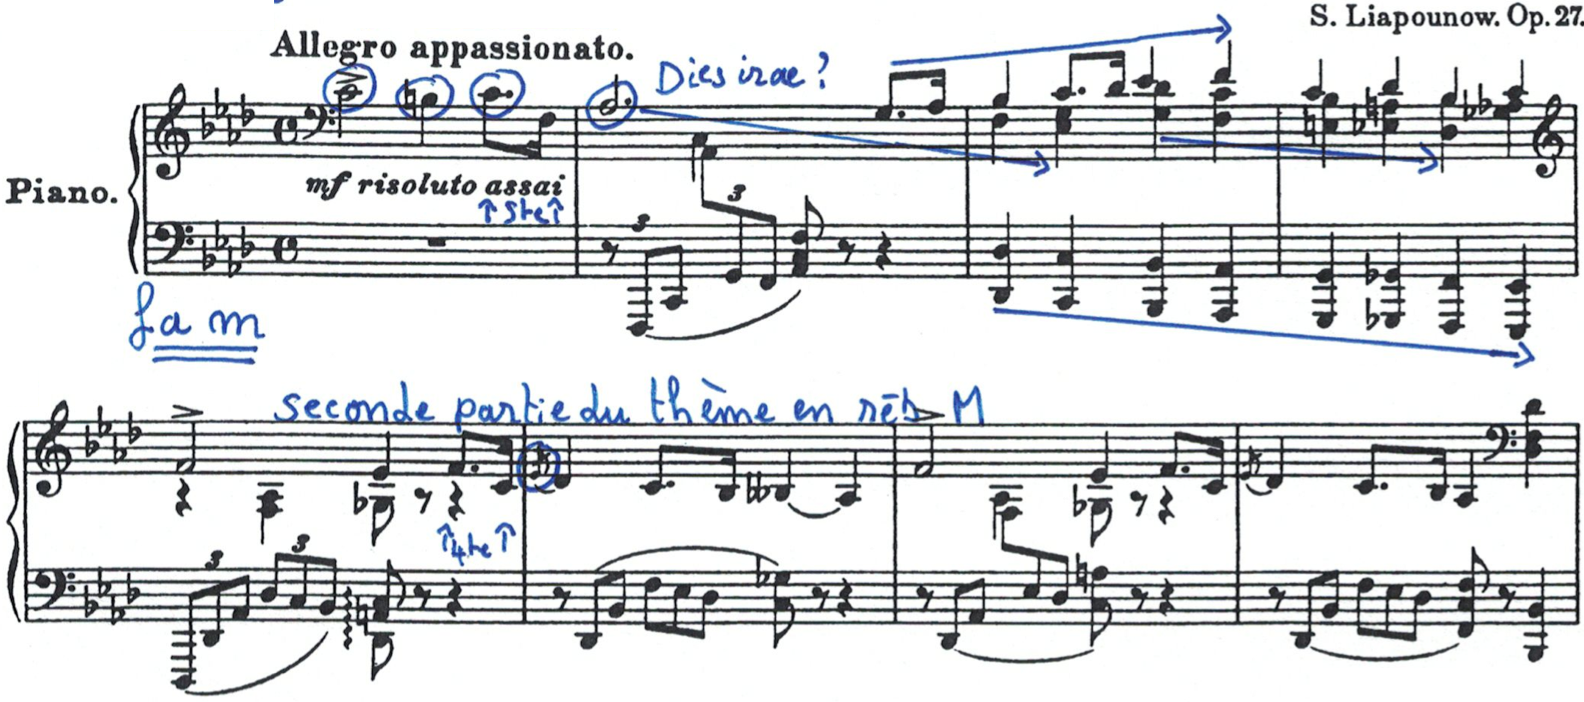
\includegraphics[width=12.5cm, keepaspectratio]{sonate-theme-A.png}
      &
      
\includegraphics[width=3cm, keepaspectratio]{op1-qr.png}
    \end{tabular}
  \end{bigcenter}
  \caption{\label{sonate-theme-1}Sonate en \emph{fa} mineur op.27, thème A.}
\end{figure}

\textbf{Le deuxième (thème B)}, apparaît page 3, mesure 52 au \emph{Cantabile ed espressivo} (voir figure \ref{sonate-theme-2}). Écrit en 6/4 et toujours en \emph{fa} mineur, il présente des similitudes avec le thème principal dont il est issu (voir figure \ref{sonate-theme-1-vs-2}). Il est néanmoins plus chantant et plaintif. L'écriture de la main gauche évoque le style pianistique de Chopin.

\begin{figure}[!ht]
  \begin{bigcenter}
    \vspace*{0.2cm}
    \begin{tabular}{lr}
      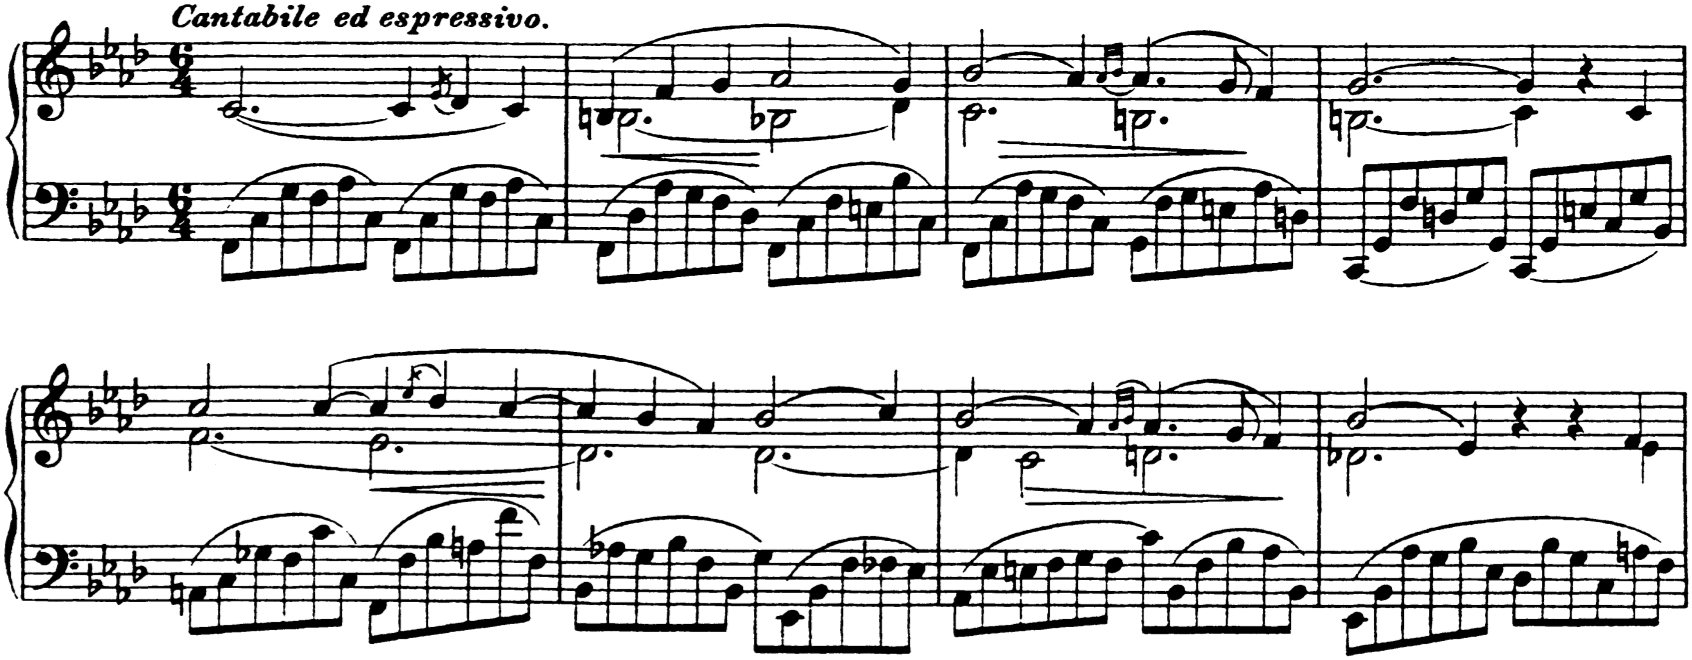
\includegraphics[width=12.5cm, keepaspectratio]{sonate-theme-B.png}
      &
      
\includegraphics[width=3cm, keepaspectratio]{op1-qr.png}
    \end{tabular}
  \end{bigcenter}
  \caption{\label{sonate-theme-2}Sonate en \emph{fa} mineur op.27, thème B.}
\end{figure}

\begin{figure}[!ht]
  \begin{bigcenter}
      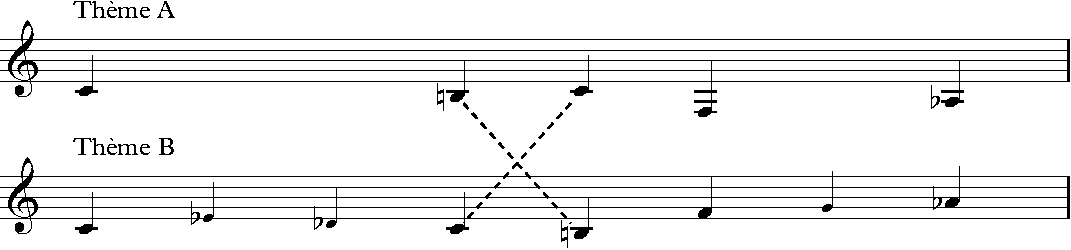
\includegraphics[width=12.75cm, keepaspectratio]{sonate-theme-A-vs-B.pdf}\vspace{-0.5cm}
  \end{bigcenter}
  \caption{\label{sonate-theme-1-vs-2}Le thème B est issu du thème A.}
\end{figure}

\textbf{Le troisième (thème C)} apparaît à la page 6, mesure 108 au \emph{Un poco meno mosso} (voir figure \ref{sonate-theme-3}). Écrit à quatre temps, sur pédale de tonique en ré majeur, il emprunte en douceur (\emph{dolcissimo molto con anima}) une pente mélodique descendante puis ascendante. Notons la liaison à la voix supérieure de la main gauche sur chaque blanche. Ici encore les deux premières mesures sont issues de la seconde partie du thème principal (voir figure \ref{sonate-theme-1-vs-3})

\begin{figure}[!ht]
  \begin{bigcenter}
    \begin{tabular}{lr}
      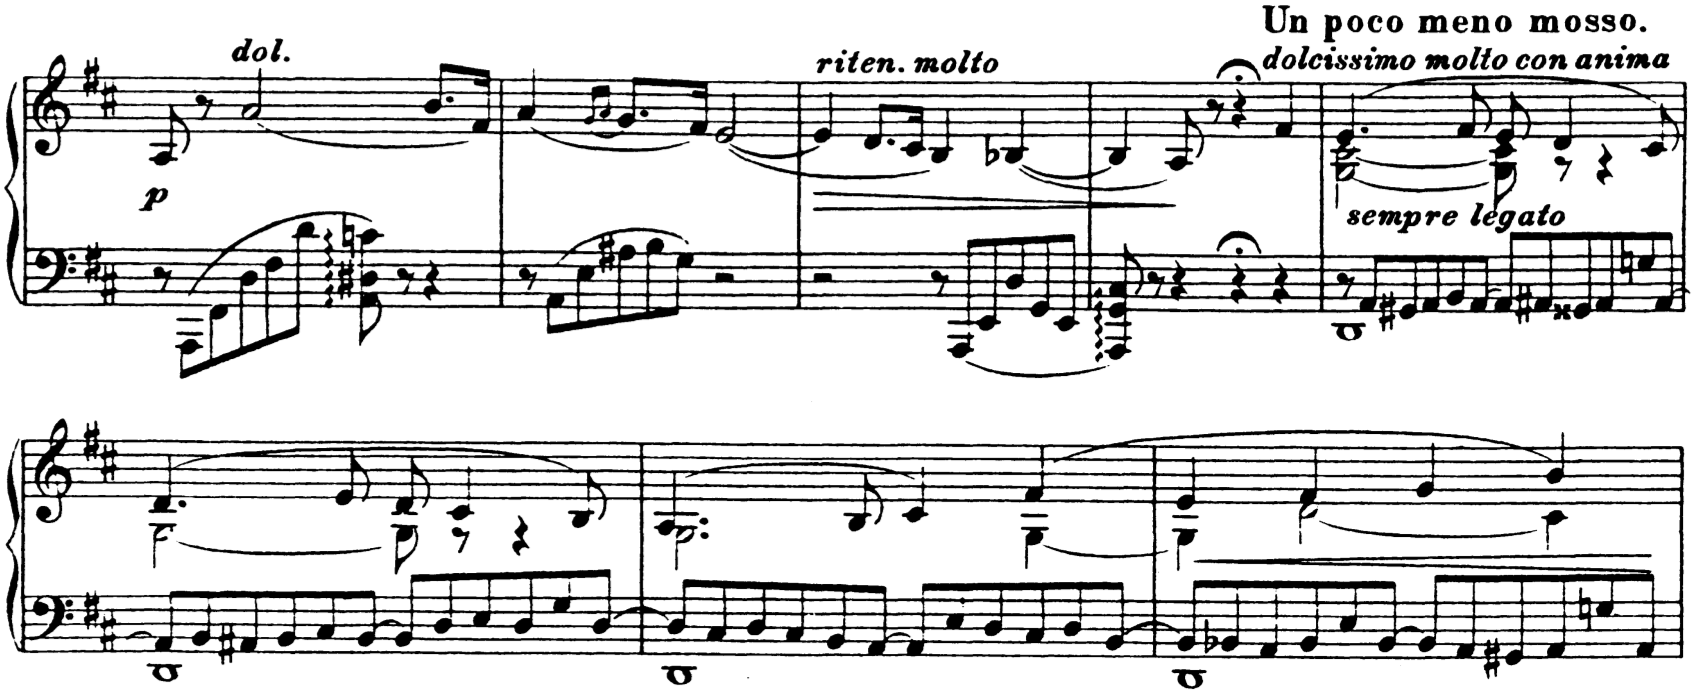
\includegraphics[width=12.5cm, keepaspectratio]{sonate-theme-C.png}
      &
      
\includegraphics[width=3cm, keepaspectratio]{op1-qr.png}
    \end{tabular}
  \end{bigcenter}
  \caption{\label{sonate-theme-3}Sonate en \emph{fa} mineur op.27, thème C.}
\end{figure}

\begin{figure}[!ht]
  \begin{bigcenter}
      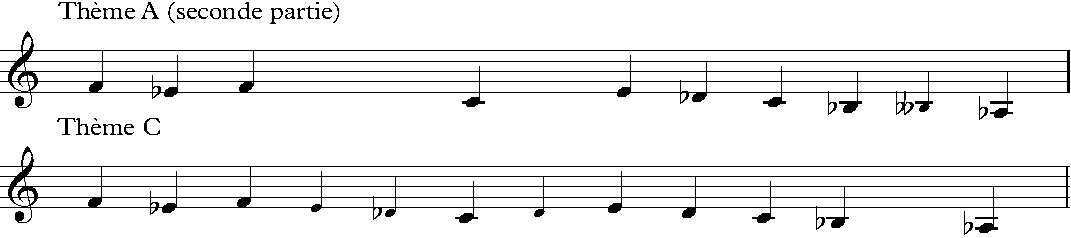
\includegraphics[width=12.75cm, keepaspectratio]{sonate-theme-A-vs-C.pdf}\vspace{-0.5cm}
  \end{bigcenter}
  \caption{\label{sonate-theme-1-vs-3}Le thème C est issu du thème A.}
\end{figure}

\textbf{Le quatrième (thème D)} apparaît au début du deuxième mouvement à la page 13, mesure 245 l'\emph{Andante sostenuto e molto espressivo} (voir figure \ref{sonate-theme-4}). Écrit à 12/8, en \emph{mi} majeur, il s'agit typiquement d'un thème de nocturne. Si on transpose la seconde partie du thème A, on constate que les deux premières notes sont communes aux deux thèmes. Il n'est pas possible d'aller plus loin dans la correspondance, cependant, on peut supposer que le thème D s'inspire des lignes descendantes des mesures 3 et 4 de la sonate (voir figure \ref{sonate-theme-1}).

\begin{figure}[!ht]
  \begin{bigcenter}
    \begin{tabular}{lr}
      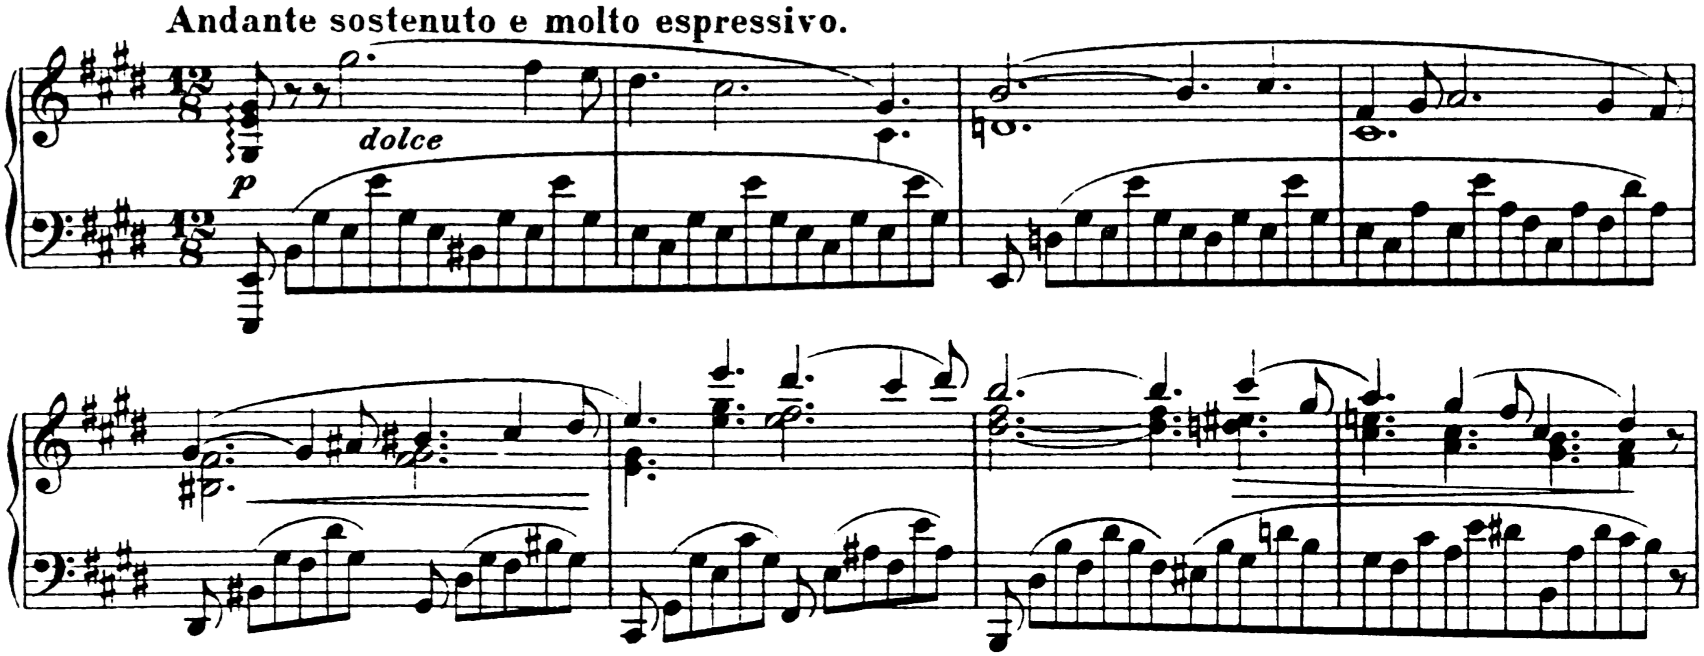
\includegraphics[width=12.5cm, keepaspectratio]{sonate-theme-D.png}
      &
      
\includegraphics[width=3cm, keepaspectratio]{op1-qr.png}
    \end{tabular}
  \end{bigcenter}
  \caption{\label{sonate-theme-4}Sonate en \emph{fa} mineur op.27, thème D.}
\end{figure}

\textbf{Le cinquième (thème E)} apparaît au centre de l'œuvre, dans le deuxième mouvement à la page 15, mesure 288 au \emph{dolcissimo} (voir figure \ref{sonate-theme-5}). Il s'agit d'un chorale liturgique russe dont on peut soligner la proximité avec la quatrième mesure du thème A ou la tête du thème C. Dans les faits, Liapounov s'est inspiré du chant \foreignlanguage{russian}{Помощник и Покровитель} (\emph{Pomoshchnik i Pokrovitel}, voir figure \ref{bortnyansky}). La réduction harmonique du thème E (voir figure \ref{sonate-theme-5-réduction}) montre l'emploi du mode dorien avec si$\flat$. Ce thème évoque également \emph{La grande porte de Kiev} de Moussorgski (voir figure \ref{grande-porte-de-kiev}).\\

\begin{figure}[!p]
  \begin{bigcenter}
    \begin{tabular}{lr}
      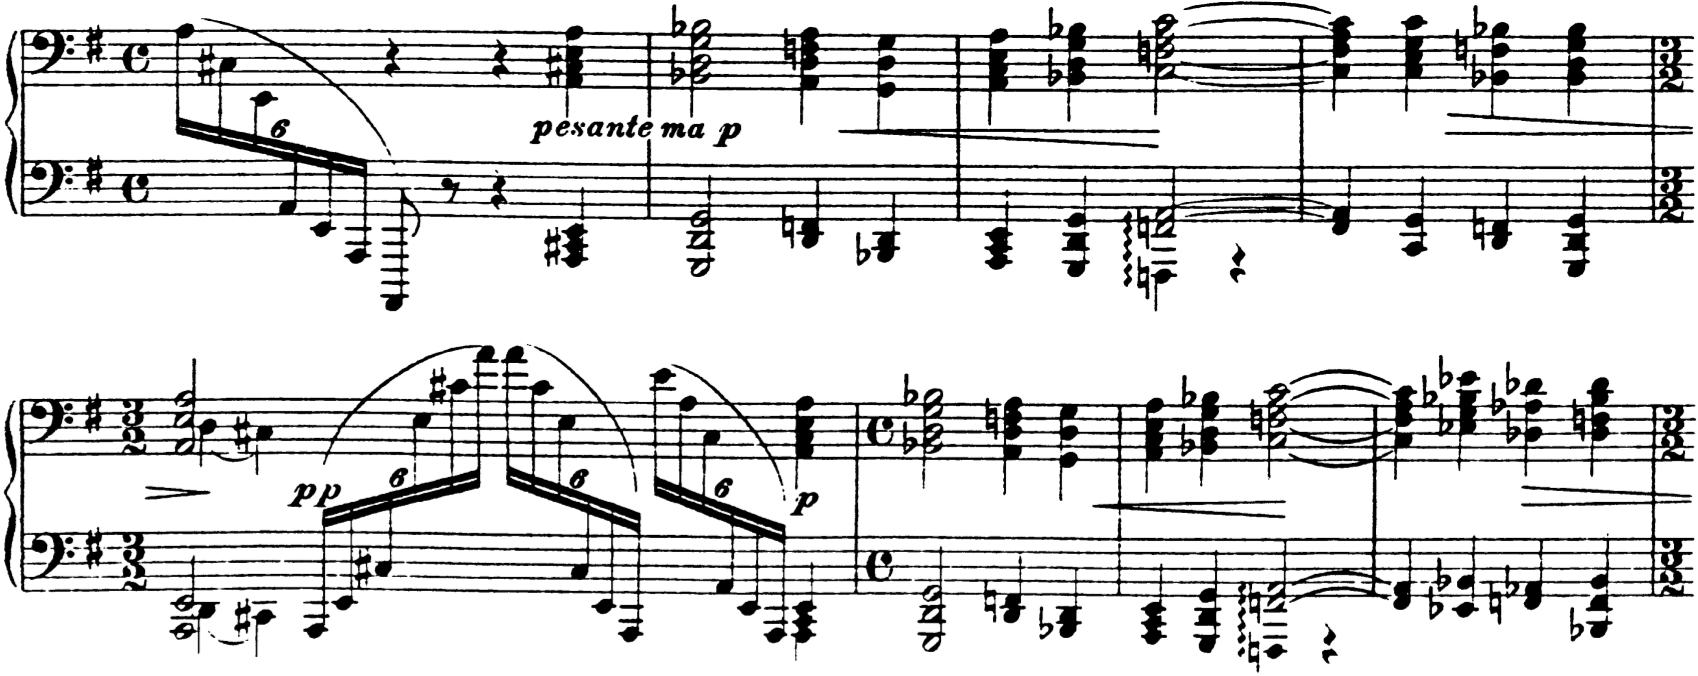
\includegraphics[width=12.5cm, keepaspectratio]{sonate-theme-E.png}
      &
      
\includegraphics[width=3cm, keepaspectratio]{op1-qr.png}
    \end{tabular}
  \end{bigcenter}
  \caption{\label{sonate-theme-5}Sonate en \emph{fa} mineur op.27, thème E.}
\end{figure}

\begin{figure}[!p]
  \begin{bigcenter}
    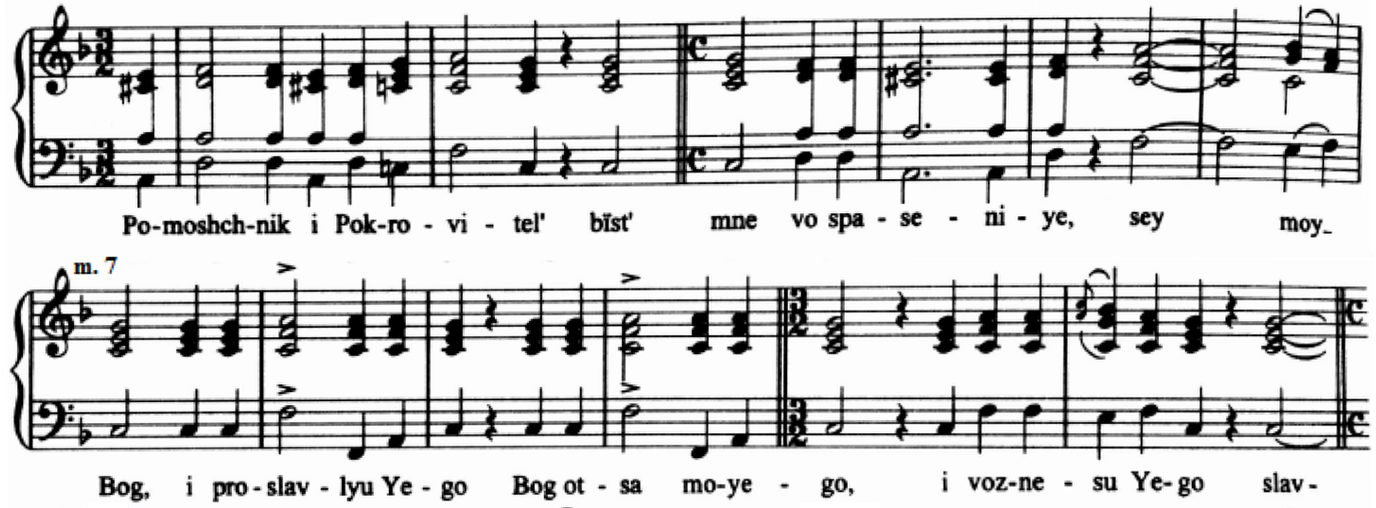
\includegraphics[width=15cm, keepaspectratio]{bortnyansky.png}
  \end{bigcenter}
  \caption{\label{bortnyansky}\foreignlanguage{russian}{Помощник и Покровитель} (\emph{Pomoshchnik i Pokrovitel}).}
\end{figure}

\begin{figure}[!p]
  \begin{bigcenter}
    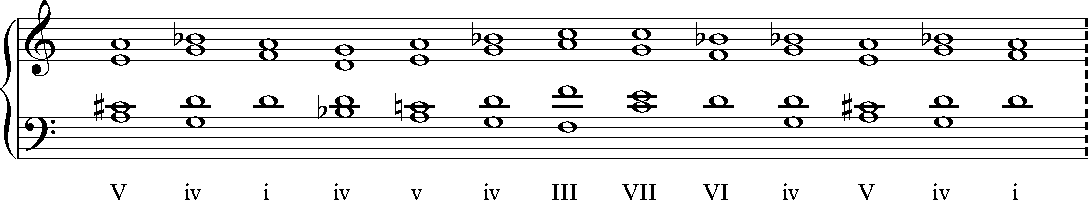
\includegraphics[width=15cm, keepaspectratio]{religioso.pdf}
  \end{bigcenter}
  \caption{\label{sonate-theme-5-reduction}Réduction harmonique du thème E (mode dorien avec si$\flat$).}
\end{figure}

\begin{figure}[!p]
  \begin{bigcenter}
    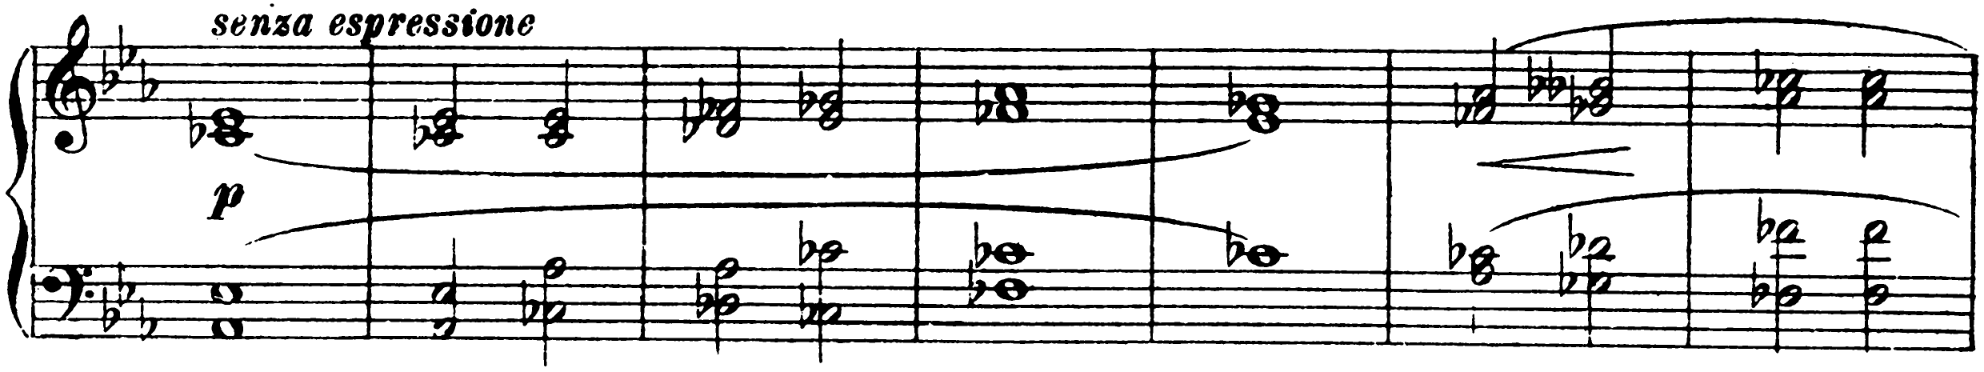
\includegraphics[width=15cm, keepaspectratio]{kiev.png}
  \end{bigcenter}
  \caption{\label{grande-porte-de-kiev}Extrait de \emph{La grande porte de Kiev} de Moussorgski.}
\end{figure}

Nous sommes en présence d'un développement continu où chaque nouveau thème émerge des précédents.\\

Remarque 1 : La tête du thème A est souvent superposée/associée à un motif ascendant en triolets voir en double croches. Même s'il s'agit d'un motif d'importance moindre, il est par la suite nommé A2 (voir figure \ref{sonate-theme-12}).\\

\begin{figure}[!ht]
  \begin{bigcenter}
    \begin{tabular}{lr}
      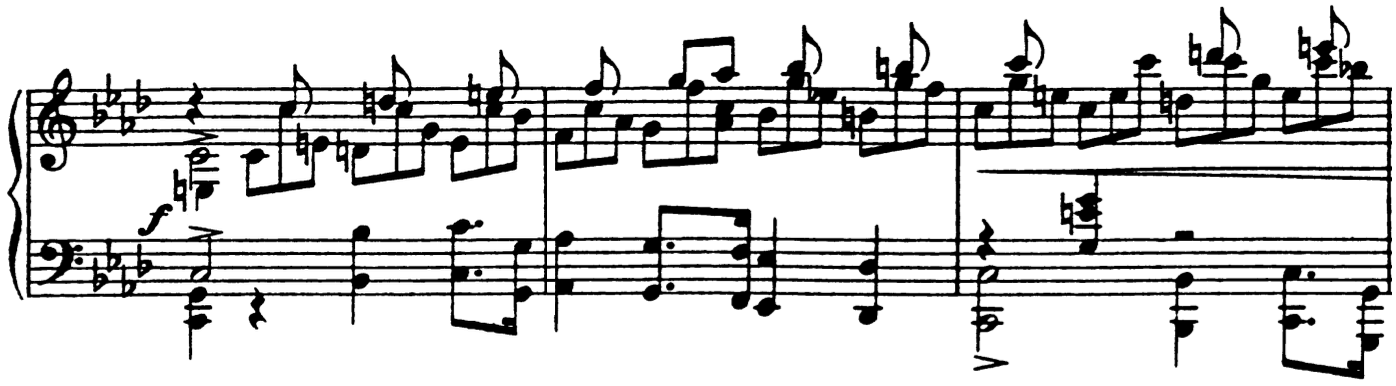
\includegraphics[width=12.5cm, keepaspectratio]{sonate-theme-A2.png}
      &
      
\includegraphics[width=3cm, keepaspectratio]{op1-qr.png}
    \end{tabular}
  \end{bigcenter}
  \caption{\label{sonate-theme-12}Sonate en \emph{fa} mineur op.27, thème A2.}
\end{figure}

Remarque 2 : On observe une certaine ambiguité entre le binaire et le ternaire. En effet, le thème A est binaire (C) mais il se superpose au thème A2 qui est la plupart du temps écrit en triolets. Le thème B est à 6/4. Le thème C est binaire mais l'accompagnement est en sextolets de croches. Le thème D est à 12/8 avec une basse de quatre fois six croches. Chaque groupe de six commence à la deuxième croche de la mesure et les appuis se décalent. La première occurrence du thème E alterne des groupes de mesure à C avec une mesure à 3/2.

\section{Analyse et forme}

Comme indiqué précédemment, nous retrouvons la structure traditionnelle d'une sonate à quatre mouvements. Analysons la structure de chacun des mouvements pris comme une entité autonome et vérifions si une structure plus globale se dégage (formes dans la forme).

\subsubsection*{Le premier mouvement (244 mesures, $\sim$9m30s)}

Le premier mouvement est le plus long et le plus complexe de la sonate. Les 51 premières mesures servent à introduire le thème A dans la tonalité principale de la sonate, c'est-à-dire fa mineur. Les 48 mesures suivantes introduisent le thème B. De façon un peu surprenante, ce thème reste en fa mineur. La raison de cela est qu'il s'agit en simplement d'un thème de transition. La page 5 mène à la petite cadence lisztienne du début de la page 6 dont le but est d'installer la tonalité de ré majeur. Le thème C est alors introduit. Il est développé, conjointement au thème A jusqu'à la grande pédale de la de la page 8. La page 9, mesure 162 est clairement ressentie comme une ré-exposition dans la tonalité de ut$\sharp$ mineur avec la thème A mesure 162, puis le thème B à la mesure 170. Cette ré-exposition se termine à la mesure 236 en ré$\flat$ majeur ($\sim$ut$\sharp$ majeur). Par enharmonie, une deuxième petite cadence lisztienne en ut$\sharp$ mineur prépare le cinquième degré de mi majeur (ton relatif), le ton de mouvement suivant.\\

Ce premier mouvement peut être vu comme une sorte de forme-sonate sans développement où l'exposition, comme la ré-exposition, exploitent suffisamment le matériau pour que l'ensemble reste consistante. La figure \ref{schema-1} résume la structure du premier mouvement.

\begin{figure}[!ht]
  \begin{bigcenter}
    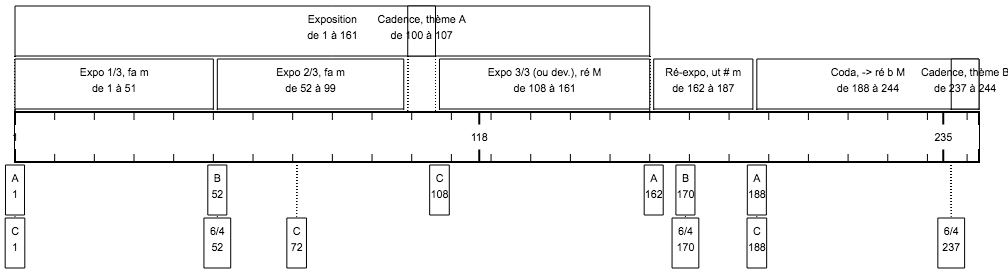
\includegraphics[width=17.5cm, keepaspectratio]{frise-mvt1.png}
  \end{bigcenter}
  \caption{\label{schema-1}Schéma du premier mouvement.}
\end{figure}

\subsubsection*{Le deuxième mouvement (118 mesures, $\sim$8m15s)}

Le deuxième mouvement à une simple forme tripartite A + B + A'. La partie A (A1 + a1) est constituée du thème D en mi majeur sur 24 mesures (A1) puis d'une section non thématique sur une pédale de la (dominante de ré) sur 18 mesures (a1). La partie B est constituée de deux répétitions variées du thème E en ré dorien sur 21 puis 23 mesures. Mesure 87, une petite cadence de 8 mesure, évoquant également le scintillement \emph{La grande porte de Kiev} de Moussorgski, ré-installe la tonalité de mi majeur. Enfin, la partie A' (A2 + a2) est constituée à nouveau du thème D en mi majeur sur 8 mesures (A2) et d'une partie conclusive qui aboutie sur la dominante (demie-cadence) de sol$\sharp$ m. La figure \ref{schema-2} résume la structure du deuxième mouvement.

\begin{figure}[!ht]
  \begin{bigcenter}
    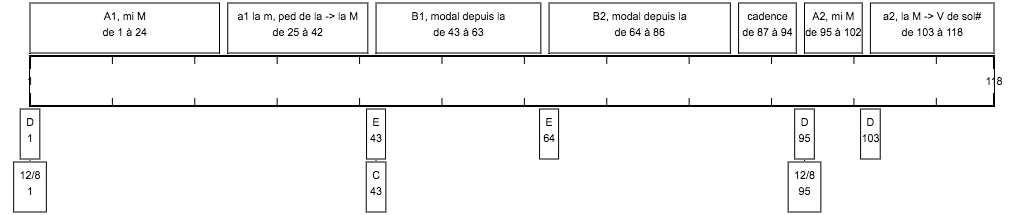
\includegraphics[width=17.5cm, keepaspectratio]{frise-mvt2.png}
  \end{bigcenter}
  \caption{\label{schema-2}Schéma du deuxième mouvement.}
\end{figure}

\subsubsection*{Le troisième mouvement (92 mesures, $\sim$2m8s)}

Dans les grandes sonates du XIX\ieme{} siècle, le troisième mouvement est très souvent un scherzo, c'est-à-dire une forme ternaire héritée du menuet, la plupart du temps à 3/4. Dans le cas de la sonate de Liapounov, nous avons trois variations en sol$\sharp$ mineur sur le thème B. Il ne s'agit pas réellement d'un scherzo mais la partition porte tout de même l'indication \emph{scherzando}. L'écriture \emph{Allegro vivo} à 6/8, au lieu de 6/4 dans le premier mouvement, confère un caractère qui volubile et rythmé. Il s'agit du plus court mouvement de la sonate.

La forme est la suivante : introduction évoquant le thème B (8 mesures, sol$\sharp$ mineur) + thème B (12 mesures, sol$\sharp$ mineur) + élément non thématique avec cadence (14 mesures, si majeur retour en sol$\sharp$ mineur) + variation ornementale du thème B (8 mesures, sol$\sharp$ mineur) + élément non thématique avec cadence (10 mesures, la majeur, retour en sol$\sharp$ mineur) + variation ornementale du thème B (8 mesures, sol$\sharp$ mineur) + élément non thématique avec cadence (12 mesures, do$\sharp$ majeur, retour vers sol$\sharp$ mineur) + codetta basée sur le thème B non varié (20 mesures, en sol$\sharp$ mineur modulant, se dirige vers fa mineur (= la tonalité principale de la sonate)). La figure \ref{schema-3} résume la structure du troisième mouvement.

\begin{figure}[!ht]
  \begin{bigcenter}
    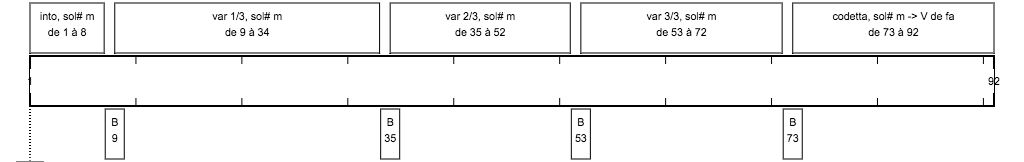
\includegraphics[width=17.5cm, keepaspectratio]{frise-mvt3.png}
  \end{bigcenter}
  \caption{\label{schema-3}Schéma du troisième mouvement.}
\end{figure}

\subsubsection*{Le quatrième mouvement (144 mesures, $\sim$7m10s)}

S'il fait office de final, nous allons voir que le dernier mouvement de la sonate de Liapounov fait également office de ré-exposition (96 premières mesures) puis de coda (48 dernières mesures). En effet, nous retrouvons tous les éléments thématiques constitutifs des trois premiers mouvements de l'œuvre. De même que dans la sonate en si mineur de Liszt (ou dans le premier concerto), il y a deux nivaux d'analyse (quatre mouvements ou un seul mouvement). Ici, nous avons clairement affaire à une forme-sonate cyclique monolithique.

\paragraph{La ré-exposition}

Celle-ci commence sur un cinquième degré de fa avec le retour, pour la première fois depuis le premier mouvement, d'une version dégradée du thème A à la basse. Les 20 premières mesures ne sont qu'une préparation au retour du fa mineur mesure 21. C'est là que commence réellement la ré-exposition avec le thème A. Le thème A2 se fait entendre mesure 25 sur un cinquième degré. Aux mesures 45 et 46, nous glissons, par modulations chromatiques successives, vers un cinquième degré de ré$\flat$ majeur. Il s'agit de la fin de la première sous-partie de la ré-exposition.

À la mesure 47 (\emph{Meno mosso}), commence le thème C en ré$\flat$ majeur puis, mesure 51, à la tierce en sol$\flat$ majeur. Les deux occurrences se font sur pédale de ré$\flat$ (pédale de tonique). Puis, le thème A se fait à nouveau entendre en ré$\flat$ majeur, puis à la seconde en mi$\flat$ mineur. Les deux occurrences sont cette fois sur pédale de la$\flat$ (pédale de dominante). Nous arrivons ensuite, mesure 63 sur le \emph{piano}, sur une grande pédale de dominante de fa qui demeurera jusqu'au \emph{Più animato} mesure 82. Cette page est le pendant de la page 8. Elle fait entendre les thèmes C et une variante de B2. Il s'agit de la fin de la deuxième sous-partie de la ré-exposition.

Le \emph{Più animato} correspond au retour en fa mineur. Il fait entendre le thème B2 puis une cadence de dix mesures jusqu'à la double barre avant le 12/8. Cette section de 14 mesure est la fin de la ré-exposition.

\newpage

\paragraph{La coda}

La coda commence au 12/8 et se termine à la fin de l'œuvre. Elle est entièrement écrite en fa majeur et se divise en deux parties. La première commence au \emph{Andante maestoso} et se termine juste avant l'\emph{L'istesso tempo} sur la demie-cadence de fa. Elle est construite sur le thème D (en mi majeur dans le deuxième mouvement). L'écriture pianistique évoque très clairement \emph{Mazeppa} dans les \emph{études d'exécution transcendante} de Liszt (voir figure \ref{sonate-coda}). La seconde et dernière partie de la coda est basée sur le thème E à partir de fa (à partir de la dans le deuxième mouvement). La sonate se termine par dix mesures de cadence parfaite en fa majeur, aussi paisiblement qu'à la fin de la sonate en si mineur de Liszt (voir figure \ref{sonate-fin}).\\

La figure \ref{schema-4} résume la structure du quatrième mouvement.

\begin{figure}[!ht]
  \begin{bigcenter}
    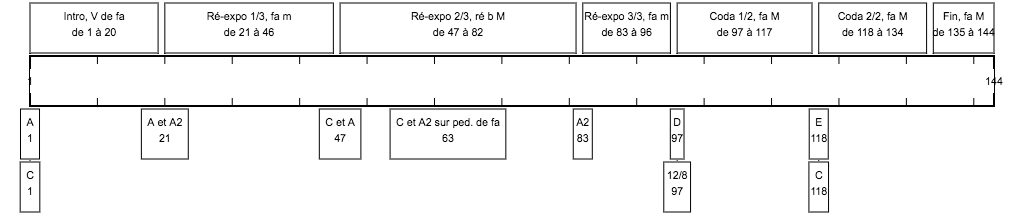
\includegraphics[width=17.5cm, keepaspectratio]{frise-mvt4.png}
  \end{bigcenter}
  \caption{\label{schema-4}Schéma du quatrième mouvement.}
\end{figure}

\begin{figure}[!p]
  \begin{bigcenter}
    \begin{tabular}{lr}
      \vspace*{0.0cm}
      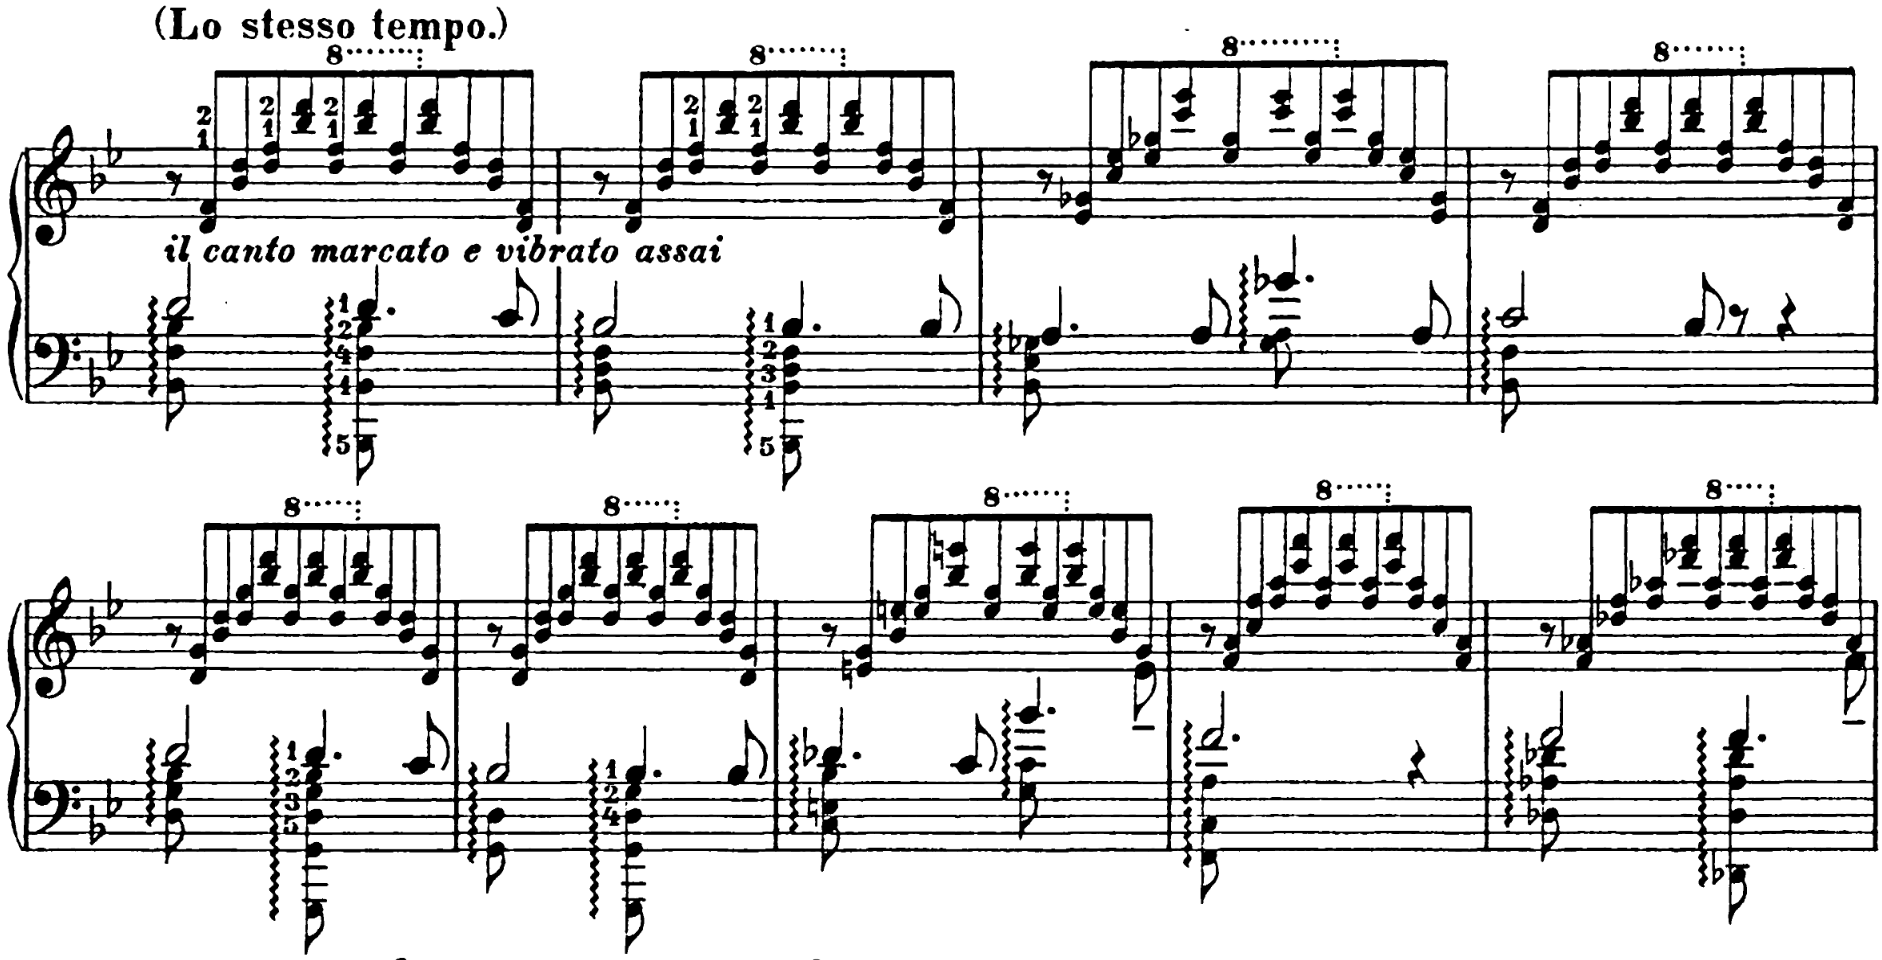
\includegraphics[width=12.5cm, keepaspectratio]{mazeppa.png}
      &
      
\includegraphics[width=3cm, keepaspectratio]{mazeppa-qr.png}
      \\
      \vspace{0.5cm} &
      \\
      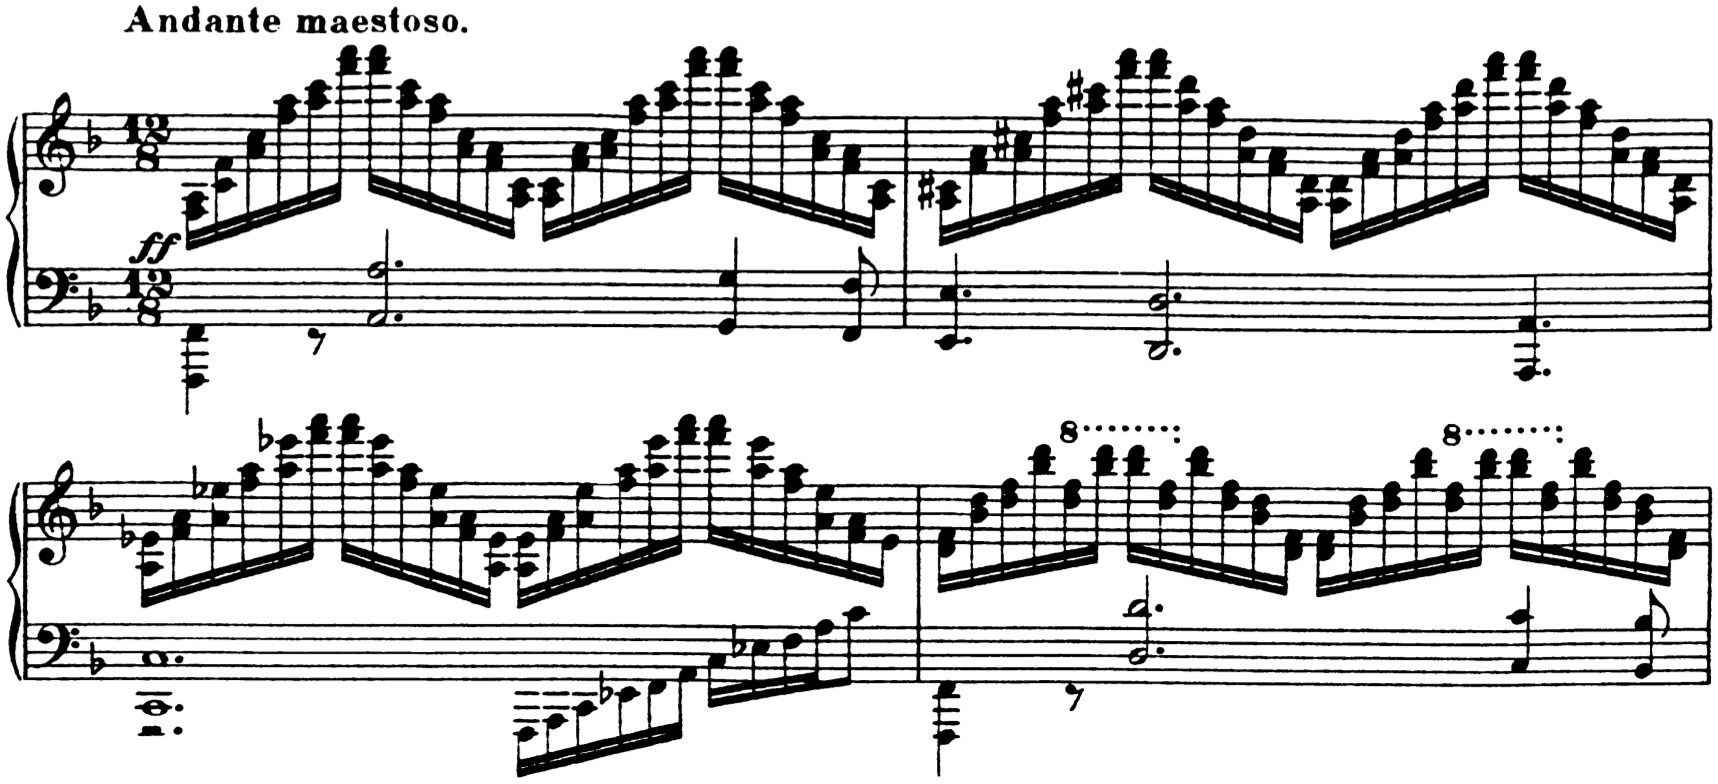
\includegraphics[width=12.5cm, keepaspectratio]{sonate-coda.png}
      &
      
\includegraphics[width=3cm, keepaspectratio]{sonate-qr.png}
    \end{tabular}
  \end{bigcenter}
  \caption{\label{sonate-coda}Comparaison de \emph{Mazeppa} de Liszt (en haut) et du début de la coda de la sonate op.27 de Liapounov (en bas).}
\end{figure}

\begin{figure}[!p]
  \begin{bigcenter}
    \begin{tabular}{lr}
      \vspace*{0.0cm}
      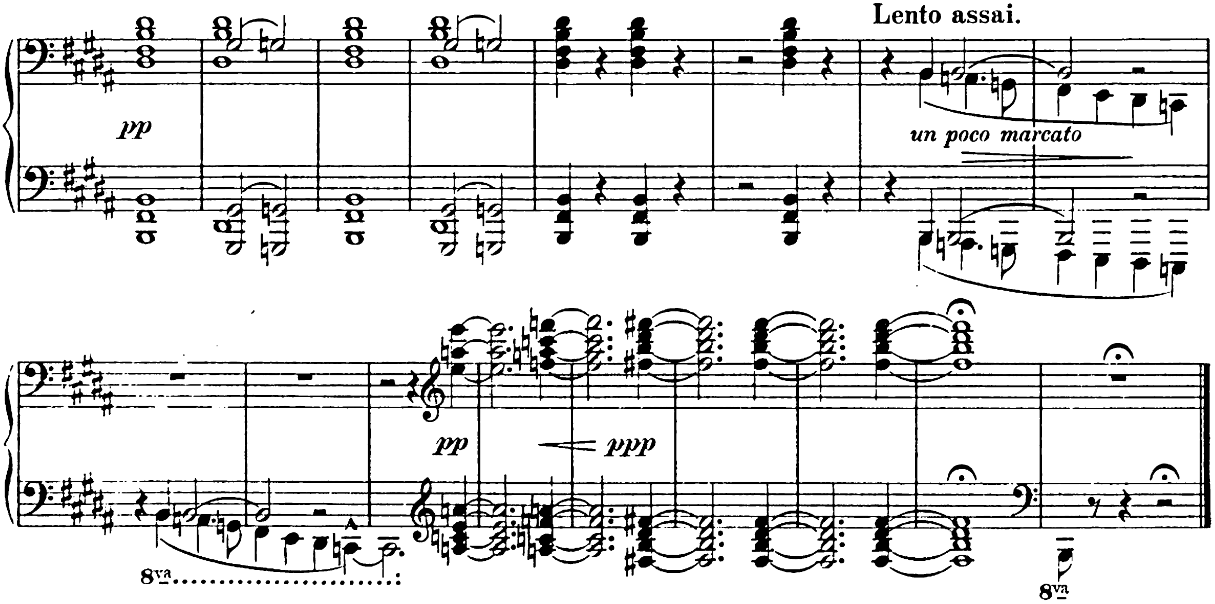
\includegraphics[width=12.5cm, keepaspectratio]{sonate-liszt-fin.png}
      &
      
\includegraphics[width=3cm, keepaspectratio]{sonate-liszt-fin-qr.png}
      \\
      \vspace{0.5cm} &
      \\
      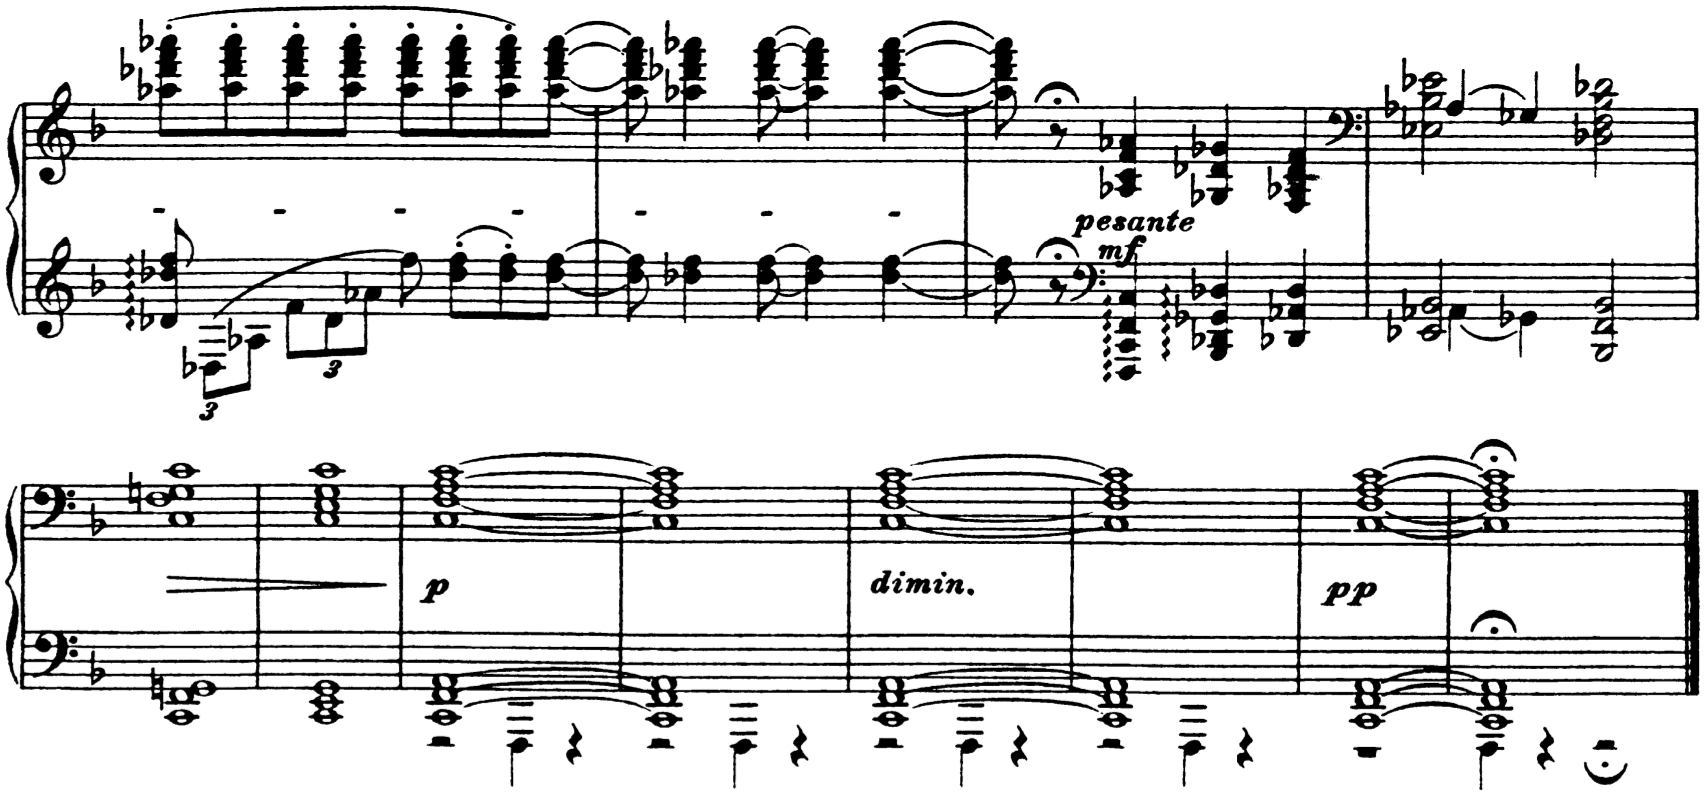
\includegraphics[width=12.5cm, keepaspectratio]{sonate-fin.png}
      &
      
\includegraphics[width=3cm, keepaspectratio]{sonate-qr.png}
    \end{tabular}
  \end{bigcenter}
  \caption{\label{sonate-fin}Comparaison de fin de la sonate S.178 de Liszt (en haut) et de la fin de la coda de la sonate op.27 de Liapounov (en bas).}
\end{figure}

\section{Deux niveaux de lecture}

Il existe donc deux niveaux de lecture, soit on considère un sonate en quatre mouvements, soit on considère un forme-sonate globale avec une exposition (mesures 1 à 161), un développement (mesures 162 à 453) et une ré-exposition (mesures 455 à 598) où les différents thèmes sont réutilisés de façon cyclique.

\begin{figure}[!p]
  \begin{bigcenter}
    \vspace{-1cm}
    \rotatebox{90} {
\begin{tabular}{|l|l|l|l|l|l|l|l|l|l|l|l|l|l|}
 \hline
   Mesures & 1 & 52 & 108 & 162 & 170 & 245 & 288 & 339 & 363 & 455 & 501 & 537 & 551 \\
 \hline
 \hline
   1 mvts & \multicolumn{13}{|l|}{Sonate cyclique}\\
 \hline
          & \multicolumn{3}{|l|}{Exposition} & \multicolumn{6}{l|}{Développement} & \multicolumn{3}{l|}{Ré-exposition} & Coda\\
 \hline
   Thème & A & B & C & \multicolumn{6}{l|}{} & A & C & B & E\\
 \hline
 \hline
   4 mvts & \multicolumn{5}{|l|}{Forme-sonate sans dév.} & \multicolumn{3}{|l|}{Forme tripartite ABA'} & variations & \multicolumn{4}{|l|}{Final}\\
 \hline
          & \multicolumn{3}{|l|}{Exposition} & \multicolumn{2}{l|}{Ré-Exposition} & \multicolumn{3}{l|}{Mvt lent} & Scherzando & \multicolumn{4}{l|}{}\\
 \hline
  Thèmes & A & B & C & A & B & D & E & D & B & A & C & B & D, E\\
 \hline
 \hline
  Signatures & C & \multicolumn{4}{|l|}{6/4, C} & 12/8 & C & 12/8 & 6/8 & \multicolumn{3}{|l|}{C} & 12/8, C\\
 \hline
  Tempos & \multicolumn{5}{|l|}{rapide} & \multicolumn{3}{|l|}{lent} & rapide & \multicolumn{3}{|l|}{rapide} & rapide/lent\\
 \hline
  Tons & fa m & fa m & ré M & \multicolumn{2}{|l|}{do$\sharp$ m} & mi M & ré m & mi M & sol$\sharp$ m & fa m & ré$\flat$ M & \multicolumn{2}{|l|}{fa M}\\
 \hline
\end{tabular}
    }
  \end{bigcenter}
  \caption{\label{structure}Structure de la sonate op.27 de Liapounov et mise en évidence des formes dans la forme.}
\end{figure}

\section{Comparaison avec la sonate de Liszt}

Outre les influences de Liszt, Chopin et de la musique russes (deuxième mouvement), il est intéressant de constater un certain nombre de similarités formelles entre la sonate op.27 de Liapounov et certaines œuvres de Liszt. Si un parallèle est possible avec le concerto op.posthume, on pense plus particulièrement à la sonate en si mineur S.178. Le tableau \ref{sonate-liapounov-list1} montre une comparaison des proportions des deux sonates. Le tableau \ref{sonate-liapounov-list2} montre une comparaison de la forme globale des deux sonates. On ne peut que constater la proximité structurelle ce ces deux forme-sonates cycliques.

\begin{figure}[!ht]
  \begin{bigcenter}
    \scalebox{0.925} {
\begin{tabular}{|l||l|l|l|l|l|}
 \hline
S.178 & Allegro 43\% & Antante 17\% & Fugato 10\% & Allegro 20\% & Coda 10\%\\
 \hline
 \hline
op.27 & Allegro 41\% & Antante 19\% & Scherzando 15\% & Tempo I 16\% & Coda 8\%\\
 \hline
\end{tabular}
    }
  \end{bigcenter}
  \caption{\label{sonate-liapounov-list1} Comparaison des proportions de la sonate S.178 de Liszt avec les proportions de la sonate op.27 de Liapounov.}
\end{figure}

\begin{figure}[!ht]
  \begin{bigcenter}
    \scalebox{0.925} {
\begin{tabular}{|l|l|l|}
 \hline
\multicolumn{3}{|l|}{Sonate S.178, Liszt}\\
 \hline
sol mineur & Introduction & Lent, rapide\\
si mineur & Exposition, premier thème & Rapide\\
ré majeur & Exposition, second thème & Modéré\\
- & Section conclusive & Rapide\\
- & Développement & Rapide\\
fa$\sharp$ majeur & ABA' & Modéré\\
si$\flat$ majeur/mi$\flat$ majeur & Fugato & Rapide\\
si mineur & Ré-exposition, premier thème & Rapide\\
si majeur & Ré-exposition, second thème & Modéré\\
- & Section conclusive & Rapide\\
si majeur & Coda & Rapide, lent\\
 \hline
 \hline
\multicolumn{3}{|l|}{Sonate op.27, Liapounov}\\
 \hline
fa mineur & Exposition, premier thème & Rapide\\
fa mineur/la$\flat$ majeur & Exposition, thème de transition & Modéré\\
ré majeur & Exposition, second thème & Modéré \\
- & Développement & Rapide\\
mi majeur & ABA' & Modéré\\
sol$\sharp$ mineur & Scherzando & Rapide\\
fa mineur & Ré-exposition, premier thème & Rapide\\
ré$\flat$ majeur & Ré-exposition, second thème & Modéré\\
- & Transition & Rapide\\
fa majeur & Coda & Modéré, lent\\
 \hline
\end{tabular}
    }
  \end{bigcenter}
  \caption{\label{sonate-liapounov-list2} Comparaison de la structure de la sonate S.178 de Liszt avec la structure de la sonate op.27 de Liapounov.}
\end{figure}

\section{Conclusion}

La sonate op.27 se présente comme un point de rencontre entre les influances européennes et les traditions russes. Elle constitue un sommet de l'œuvre de Liapouov mais aussi un sommet pour les sonates russes du début du XX\ieme{} siècle.

Stylistiquement, les courbes évoquent le pianisme de Chopin et le choral liturgique du deuxième mouvement est dans l'estétique de Balakirev et du \emph{Groupe des Cinq}. Structurellement, la connection avec la sonate en si mineur S.178 de Liszt est évidente. Les deux œuvres partagent les même proportions et une structure très proche. Nous sommes en présence de deux forme-sonates cycliques en un seul mouvement.

%%%%%%%%%%%%%%%%%%%%%%%%%%%%%%%%%%%%%%%%%%%%%%%%%%%%%%%%%%%%%%%%%%%%%%%%%%%%%
